\documentclass[]{article}
\usepackage{lmodern}
\usepackage{amssymb,amsmath}
\usepackage{ifxetex,ifluatex}
\usepackage{fixltx2e} % provides \textsubscript
\ifnum 0\ifxetex 1\fi\ifluatex 1\fi=0 % if pdftex
  \usepackage[T1]{fontenc}
  \usepackage[utf8]{inputenc}
\else % if luatex or xelatex
  \ifxetex
    \usepackage{mathspec}
  \else
    \usepackage{fontspec}
  \fi
  \defaultfontfeatures{Ligatures=TeX,Scale=MatchLowercase}
\fi
% use upquote if available, for straight quotes in verbatim environments
\IfFileExists{upquote.sty}{\usepackage{upquote}}{}
% use microtype if available
\IfFileExists{microtype.sty}{%
\usepackage{microtype}
\UseMicrotypeSet[protrusion]{basicmath} % disable protrusion for tt fonts
}{}
\usepackage[margin=1in]{geometry}
\usepackage{hyperref}
\hypersetup{unicode=true,
            pdftitle={AquaSat Supplementary Information},
            pdfborder={0 0 0},
            breaklinks=true}
\urlstyle{same}  % don't use monospace font for urls
\usepackage{graphicx,grffile}
\makeatletter
\def\maxwidth{\ifdim\Gin@nat@width>\linewidth\linewidth\else\Gin@nat@width\fi}
\def\maxheight{\ifdim\Gin@nat@height>\textheight\textheight\else\Gin@nat@height\fi}
\makeatother
% Scale images if necessary, so that they will not overflow the page
% margins by default, and it is still possible to overwrite the defaults
% using explicit options in \includegraphics[width, height, ...]{}
\setkeys{Gin}{width=\maxwidth,height=\maxheight,keepaspectratio}
\IfFileExists{parskip.sty}{%
\usepackage{parskip}
}{% else
\setlength{\parindent}{0pt}
\setlength{\parskip}{6pt plus 2pt minus 1pt}
}
\setlength{\emergencystretch}{3em}  % prevent overfull lines
\providecommand{\tightlist}{%
  \setlength{\itemsep}{0pt}\setlength{\parskip}{0pt}}
\setcounter{secnumdepth}{0}
% Redefines (sub)paragraphs to behave more like sections
\ifx\paragraph\undefined\else
\let\oldparagraph\paragraph
\renewcommand{\paragraph}[1]{\oldparagraph{#1}\mbox{}}
\fi
\ifx\subparagraph\undefined\else
\let\oldsubparagraph\subparagraph
\renewcommand{\subparagraph}[1]{\oldsubparagraph{#1}\mbox{}}
\fi

%%% Use protect on footnotes to avoid problems with footnotes in titles
\let\rmarkdownfootnote\footnote%
\def\footnote{\protect\rmarkdownfootnote}

%%% Change title format to be more compact
\usepackage{titling}

% Create subtitle command for use in maketitle
\providecommand{\subtitle}[1]{
  \posttitle{
    \begin{center}\large#1\end{center}
    }
}

\setlength{\droptitle}{-2em}

  \title{AquaSat Supplementary Information}
    \pretitle{\vspace{\droptitle}\centering\huge}
  \posttitle{\par}
    \author{}
    \preauthor{}\postauthor{}
      \predate{\centering\large\emph}
  \postdate{\par}
    \date{May 16, 2019}

\usepackage{booktabs}
\usepackage{longtable}
\usepackage{array}
\usepackage{multirow}
\usepackage{wrapfig}
\usepackage{float}
\usepackage{colortbl}
\usepackage{pdflscape}
\usepackage{tabu}
\usepackage{threeparttable}
\usepackage{threeparttablex}
\usepackage[normalem]{ulem}
\usepackage{makecell}
\usepackage{xcolor}

\begin{document}
\maketitle

\hypertarget{tables}{%
\section{Tables}\label{tables}}

\begin{table}[t]

\caption{\label{tab:landsat}Summary of landsat wavelengths and resolution. Bands with an asterisk* indicate that they were not used in this project. Note that panchromatic 
        band is only available for top of atmosphere data, not surface reflectance}
\centering
\begin{tabu} to \linewidth {>{\raggedright}X>{\raggedright}X>{\raggedright}X>{\raggedright}X>{\raggedright}X}
\hline
\textbf{Bands} & \textbf{L5 Wavelengths} & \textbf{L7 Wavelengths} & \textbf{L8 Wavelengths} & \textbf{Resolution (m)}\\
\hline
Blue & 0.45-0.52 & 0.45-0.52 & 0.452-0.512 & 30\\
\hline
Green & 0.52-0.60 & 0.52-0.60 & 0.533-0.590 & 30\\
\hline
Red & 0.63-0.69 & 0.63-0.69 & 0.636-0.673 & 30\\
\hline
Near Infrared (nir) & 0.77-0.90 & 0.77-0.90 & 0.851-0.879 & 30\\
\hline
Shortwave Infrared 1(swir1) & 1.55-1.75 & 1.55-1.75 & 1.566-1.651 & 30\\
\hline
Shortwave Infrared 2 (swir2) & 2.09-2.35 & 2.09-2.35 & 2.107-2.294 & 30\\
\hline
Panchromatic & NA & 0.52-0.9 & 0.503-0.676 & 15\\
\hline
Thermal* & 10.4-12.5 & 10.4-12.5 & NA & 30\\
\hline
Cirrus* & NA & NA & 1.363-1.384 & 30\\
\hline
Thermal (TIRS) 1* & NA & NA & 10.60-11.19 & 30\\
\hline
Thermal (TIRS) 2* & NA & NA & 11.50,12.51 & 30\\
\hline
\end{tabu}
\end{table}

\begin{table}[t]

\caption{\label{tab:paramters}Table shows the charactersticNames used in our WQP data download.}
\centering
\begin{tabular}{>{\raggedright\arraybackslash}p{2cm}|>{\raggedright\arraybackslash}p{13cm}}
\hline
\textbf{parameter} & \textbf{WQP characteristicNames}\\
\hline
\rowcolor{gray!6}  cdom & Colored dissolved organic matter (CDOM)\\
\hline
chlorophyll & Chlorophyll; Chlorophyll A; Chlorophyll a; Chlorophyll a (probe relative fluorescence); Chlorophyll a (probe); Chlorophyll a - Periphyton (attached); Chlorophyll a - Phytoplankton (suspended); Chlorophyll a, corrected for pheophytin; Chlorophyll a, free of pheophytin; Chlorophyll a, uncorrected for pheophytin; Chlorophyll b; Chlorophyll c; Chlorophyll/Pheophytin ratio\\
\hline
\rowcolor{gray!6}  doc & Organic carbon; Total carbon; Hydrophilic fraction of organic carbon; Non-purgeable Organic Carbon (NPOC)\\
\hline
secchi & Depth, Secchi disk depth; Depth, Secchi disk depth (choice list); Secchi Reading Condition (choice list); Secchi depth; Water transparency, Secchi disc\\
\hline
\rowcolor{gray!6}  tss & Total suspended solids; Suspended sediment concentration (SSC); Suspended Sediment Concentration (SSC); Total Suspended Particulate Matter; Fixed suspended solids\\
\hline
\end{tabular}
\end{table}

\pagebreak

\hypertarget{supplemental-figures}{%
\section{Supplemental Figures}\label{supplemental-figures}}

\begin{figure}
\centering
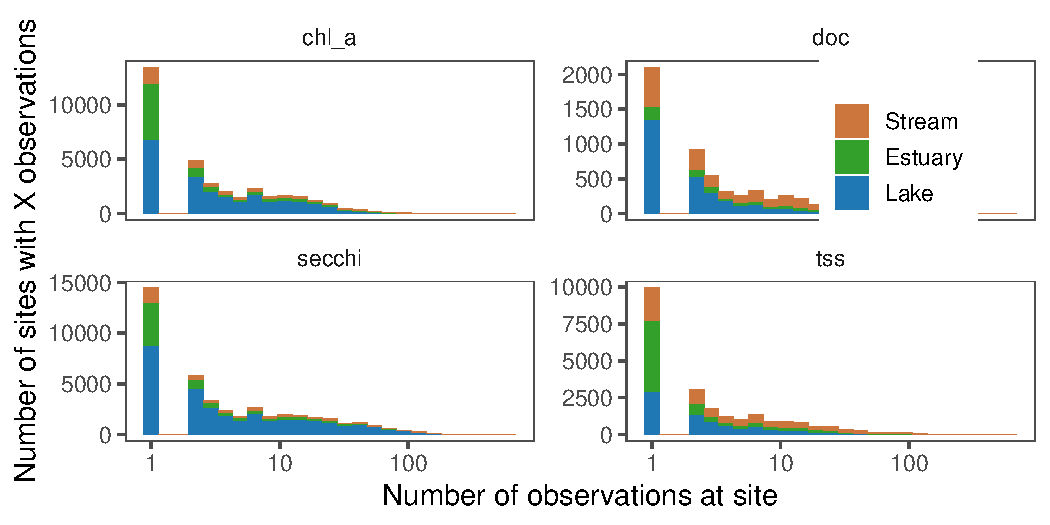
\includegraphics{AquaSat_SI_files/figure-latex/distribution-1.pdf}
\caption{\label{fig:distribution} Shows the distribution of observations
at a given site. Most sites only have a single overpass observation, but
there are thousands of these sites}
\end{figure}

\begin{figure}
\centering
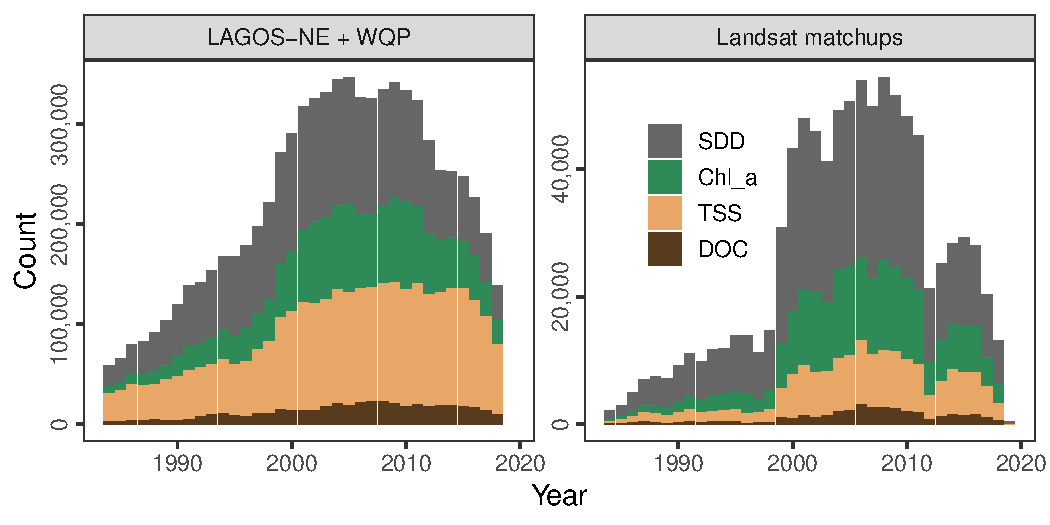
\includegraphics{AquaSat_SI_files/figure-latex/time-1.pdf}
\caption{\label{fig:time} Shows the number of observations per year per
parameter type. Note the different y axes, highlighting roughly an order
of magnitude less matchup data than incoming data. The matchup data
shows increased data availability when two satellites are in orbit.}
\end{figure}


\end{document}
